\documentclass{beamer}
\usepackage{enumerate}
\usepackage{amsmath}
\usepackage{graphicx}
\graphicspath{ {latex_figures/} }
\usepackage{booktabs,tabularx}
    \newcolumntype{L}{>{\raggedright\arraybackslash}X}
% \usepackage{beamerthemesplit} // Activate for custom appearance

\begin{document}

\title{\LARGE{Correcting Multiple Comparison Problems}}
\author{Park, Si Hyung}
\institute{Division of Life Sciences, Korea Univ.}
\date{December, 2017}
\frame{\titlepage}

\section[Outline]{}
\frame{\tableofcontents}
{
  \section{Multiple Comparison Problem}
    \subsection{Multiple Comparison Problem}
    \subsection{Multiple Comparison correction}
  \section{Family-wise Error Rate}
    \subsection{Bonferroni}
    \subsection{Holm, Hochberg}
  \section{False Discovery Rate}
    \subsection{Benjamini and Hochberg}
    \subsection{Benjamini and Yekutieli}
    \subsection{Local FDR}
  \section{Simulation \& Comparison}
}

\frame
{
  \frametitle{\LARGE{Multiple Comparison Problem}}
    Also known as "multiple hypothesis testing".\vspace{0.05in}\\
    Occurs when simultaneously making inference about a set of hypothesis
    \vspace{0.2in}\\
    
    \begin{block}{e.g. Efficacy of drug}
    \center $H_{0_1}:$ not effective to patient 1\\
    $H_{0_2}:$ not effective to patient 2\\
    ...\\
    $H_{0_m}:$ not effective to patient m\vspace{0.15in}\\
    \end{block}
    
    Family-level hypothesis is: "Is drug effective to the patients?"\\
    If level of individual hypothesis is 0.05, then family-wise error rate is $1-(1-0.05)^m > 0.05$
}

\frame
{
  \frametitle{Multiple Comparison Correction}
    Controlling error rate of a family-level hypothesis.\vspace{0.2in}\\
    Two different major types of error rate in MCP correction:
    \begin{itemize}
      \item FWER: probability of at least one type I error occurs in each individual hypothesis testing
      \item FDR: expected proportion of false positive to positives\vspace{0.2in}\\
    \end{itemize}
}

\frame
{
  \frametitle{Multiple Comparison Correction}
    Initiated by J. Tukey (1949) and H. Scheff\'e (1953), on pair-wise comparison of multiple sample means.\vspace{0.2in}\\
    
    Early works utilized $t$ or multivariate normal statistics.\vspace{0.1in}\\
    After Bonferroni procedure was developed, p-values were used.
}

\frame
{
  \frametitle{Notations - testing hypotheses}
    \begin{table}
    \small
    \setlength{\tabcolsep}{3pt}
\begin{tabularx}{\hsize}{@{}l LLL@{}}
    \toprule
 & Declared as non-significant  & Declared as significant & Total \\
    \midrule
True $H_0$ 
    & $U$ 
        & $V$ 
            & $m_0$ \\
False $H_0$ 
    & $T$ 
        & $S$
            &  $m_1=m-m_0$   \\
  
Total & $m-R$ 
        & $R$ 
            & $m$     \\
    \bottomrule
\end{tabularx}
\caption{notation of number of hypothesis in corresponding to each cell}
    \end{table}
    $R$ is an observable random variable.\vspace{0.1in}\\
    $U, V, S, T$ are unobservable random variables.
}


% FWER
\frame
{
  \frametitle{\LARGE{Family-wise Error Rate (FWER)}}
    Probability that at least one type I error occurs in individual hypothesis testing.\vspace{0.1in}\\
    \begin{itemize}
      \item $\leftrightarrow$ experiment-wise error rate\vspace{0.1in}\\
      \item $P(V\geq1)=1-P(V=0)$\vspace{0.1in}\\
      \item If $FWER \leq \alpha$, then probability of one or more type I error of the family is controlled at level $\alpha$ \vspace{0.1in}\\
    \end{itemize}
    Tukey, Scheff\'e, Dunn, $...$ contributed to FWER controlling method
}

\frame
{
  \frametitle{Bonferroni procedure}
    Tukey (1949) and Scheff\'e (1953) invented pairwise comparison method for sample means, both utilize t-statistics.\vspace{0.07in}\\
    However It's cumbersome to use these methods in MCP based on other test statistics.\vspace{0.22in}\\
    Bonferroni procedure was suggested by O. J. Dunn (1961), named after Bonferroni's inequality (generalized Boole's inequality).\vspace{0.07in}\\
Bonferroni procedure uses \underline{per-hypothesis p-values} to control FWER, rather than a specific test statistic.
}

\frame
{
  \frametitle{Bonferroni procedure}
    Suppose there is a set of $m$ hypotheses. We want to test the family-wise hypothesis with level $\alpha$.\vspace{0.07in}\\
    By testing per-hypothesis on level $\alpha \over m$, we can control $FWER \leq \alpha$.\vspace{0.22in}\\
    \begin{block}{Proof}
      By Boole's inequality: $P(\cup_{i=1}^{m}E_i)\leq\sum_{i=1}^m P(E_i)$\vspace{0.07in},\\
      \center $FWER=P(\cup_{i=1}^{m_0}(p_i\leq\dfrac{\alpha}{m}))\leq\sum_{i=1}^{m_0}P(p_i\leq\dfrac{\alpha}{m})=m_0\dfrac{\alpha}m\leq\alpha$
    \end{block}
}

\frame
{
  \frametitle{Bonferroni procedure}
    Suppose $p_i$ is a p-value of individual hypothesis $H_{0_i}$ in hypothesis family. Then, "Bonferronied" or Adjusted p-value\\ \center $p_i^{adj} = p_i \times m$.\vspace{0.1in}\\
    \flushleft Note that interpretation of adj. p-value is way different than that of original p-value.
    \begin{itemize}
      \item $p_i^{adj} \leq 0.05$: can reject $H_{0_i}$ while controlling for $FWER \leq 0.05$
      \item $p_i \leq 0.05$: probability of type I error is less than 0.05.\vspace{0.22in}\\
    \end{itemize}
}

\frame
{
    \frametitle{Bonferroni procedure}
    Pros
    \begin{itemize}
      \item Do not need assumption of dependence
      \item Remarkably simple and computationally efficient\vspace{0.1in}\\
    \end{itemize}
    
    Cons
    \begin{itemize}
      \item \textbf{Excessive amount of loss in testing power}\\ (too conservative)
    \end{itemize}
}


\frame
{
    \frametitle{Holm procedure}
    \begin{itemize}
      \item One of the first sequential (step-wise) algorithms (1979).\vspace{0.1in}
      \item Holm procedure is especially, a \underline{step-down algorithm}\vspace{0.22in}\\
      \item Uniformly more powerful than Bonferroni procedure, while controlling for FWER in strong sense.\\
    \end{itemize}
}

\frame
{
    \frametitle{Holm procedure}
    \begin{enumerate}
  \item Sort p-values in increasing order: $p_{(1)}, p_{(2)}, ..., p_{(m)}$.
    \begin{enumerate}[-]
    \item Each of the p-value corresponds to $H_{0_{(1)}}, H_{0_{(2)}}, ..., H_{0_{(m)}}$. 
    \end{enumerate}
  \item Find the smallest $j$, in which $p_{(j)} > \dfrac{\alpha}{m-j+1}$.
  \item Reject $H_{0_{(k)}}$'s, where $k=1, 2, ..., (j-1)$.\vspace{0.22in}\\
  \end{enumerate}  
  "Stepping down" the indices until we find the smallest $j$.\vspace{0.1in}\\
  Adjusted p-value: $p_{(i)}^{adj}=(m-i+1)\times p_{(i)}$\\
}

\frame
{
    \frametitle{Holm procedure}
    \begin{block}{Proof}
      Let $I$ be the set of indices of the true $H_0$'s. then length of $I$ is $m_0$.\vspace{0.07in}\\
      If the smallest index which satisfies $p_{(j)} > \dfrac{\alpha}{m-j+1}$ is $j$, then
      \center $m-j+1 \geq m_0,\text{ } \dfrac{1}{m-j+1} \leq \dfrac{1}{m_0}$\\
      $p_{(j-1)} \leq \dfrac{\alpha}{m-j+2} \leq \dfrac{\alpha}{m_0}$
      \flushleft
      By Boole's inequeality,\\
      \center $\therefore P(\cup_{i=1}^{m_0}(p_i\leq\dfrac{\alpha}{m_0}))\leq\sum_{i=1}^{m_0}P(p_i\leq\dfrac{\alpha}{m_0})=\alpha$ \vspace{0.07in} \flushleft
      Thus, FWER is controlled at level $\alpha$.
    \end{block}
}


\frame
{
    \frametitle{Holm procedure}
    \begin{itemize}
      \item Do not need assumption of dependence. \vspace{0.1in}\\
      \item Holm procedure compares individual p-values with $\dfrac{\alpha}{m}, \dfrac{\alpha}{m-1}, ..., \dfrac{\alpha}{1}$, which leads to power increase. \vspace{0.1in}\\
      \item Holm procedure is uniformly more powerful than Bonferroni procedure.
    \end{itemize}
}

\frame
{
    \frametitle{Hochberg procedure}
    Sharpened from Holm or Sime's method \vspace{0.1in}\\
    \underline{Step-up algorithm} (1988) \vspace{0.2in}\\
    \begin{enumerate}
  \item Sort p-values in increasing order: $p_{(1)}, p_{(2)}, ..., p_{(m)}$.
    \begin{enumerate}[-]
    \item Each of the p-value corresponds to $H_{0_{(1)}}, H_{0_{(2)}}, ..., H_{0_{(m)}}$. 
    \end{enumerate}
  \item Find the \textbf{largest} $j$, in which $p_{(j)} \leq \dfrac{\alpha}{m-j+1}$.
  \item Reject $H_{0_{(k)}}$'s, where $k=1, 2, ..., j$.\vspace{0.22in}\\
  \end{enumerate}  
  Uniformly more powerful than Holm procedure. \vspace{0.07in}\\
  However, needs \textbf{non-negative dependence} assumption. \\
  (as $p_{(i)}$ increases, probability of being part of true null increases)
}


\frame
{
    \center \Large{Benjamini and Hochberg introduced a seminal\\ concept, "False Discovery Rate" at 1995.} \vspace{0.2in}\\
    \flushleft \normalsize In many cases, we do not have to control FWER, especially when we want to explore as many potential effects as possible. \vspace{0.1in}\\
    FDR controls for \underline{"the ratio of erroneous rejection to all rejected} \underline{hypothesis"}, instead of probability of at least one type I error.
}


% FALSE DISCOVERY RATE
\frame
{
  \frametitle{\LARGE{False Discovery Rate (FDR)}}
    \normalsize
    FDR $Q_e$: Expectation of proportion of 'falsely rejected nulls ($V$)' to 'rejected nulls ($R$)'. \vspace{0.1in}\\
    \begin{itemize}
      \item $FDR$ $Q_e=E(Q)=E(V/R)=E(V/(V+S))$ \vspace{0.1in}\\
      \item If $m_0=m$, then $FDR=FWER$\\
        $\because s=0$, $v=r$. $P(V \geq 1)= E(Q)$\vspace{0.1in}\\
      \item If $m_0<m$, then $FDR \leq FWER$\\
        $\because v>0$, $Q \leq I_{V \geq 1}$, $E(Q) \leq E(I_{V \geq 1}) = P(V \geq 1)$ \vspace{0.2in}\\
    \end{itemize}
    Instead of "$p$", we use "$q$" to denote the level of FDR.\vspace{0.1in}\\
    Benjamini and Hochberg founded the concept of FDR (1995). 
}


\frame
{
  \frametitle{\LARGE{False Discovery Rate (FDR)}}
    \begin{block}{When to use FDR?}
    $ $ \vspace{0.05in}\\
    \begin{itemize}
      \item Family-wise conclusion is not sensitive to individual failure. \vspace{0.1in}\\
      \item Exploratory analysis. \vspace{0.1in}\\
      \item Screening for potential discoveries. \\
    \end{itemize}
    \end{block}
}


\frame
{
    \frametitle{B-H procedure}
    Benjamini and Hochberg (1995), step-up algorithm \vspace{0.2in}\\
    \begin{enumerate}
  \item Sort p-values in increasing order: $p_{(1)}, p_{(2)}, ..., p_{(m)}$.
    \begin{enumerate}[-]
    \item Each of the p-value corresponds to $H_{0_{(1)}}, H_{0_{(2)}}, ..., H_{0_{(m)}}$. 
    \end{enumerate}
  \item Find the largest $j$, in which $p_{(j)} \leq \dfrac{j}{m}q^*$, where $q^*$ is a level to control FDR for.
  \item Reject $H_{0_{(k)}}$'s, where $k=1, 2, ..., j$.\vspace{0.22in}\\
  \end{enumerate}  
  Compares $p_{(i)}$ to linear form of constant ($\propto i$) instead of hyperbolic form ($\propto \dfrac{1}{i}$), which leads to power increase.\vspace{0.07in}\\
  Needs non-negative dependence assumption.\\
}

\frame
{
    \frametitle{B-Y procedure}
    Benjamini and Yekutieli (2001), for other forms of dependency. \vspace{0.2in}\\
    \begin{enumerate}
  \item Sort p-values in increasing order: $p_{(1)}, p_{(2)}, ..., p_{(m)}$.
    \begin{enumerate}[-]
    \item Each of the p-value corresponds to $H_{0_{(1)}}, H_{0_{(2)}}, ..., H_{0_{(m)}}$. 
    \end{enumerate}
  \item Find the largest $j$, in which $p_{(j)} \leq \dfrac{j}{m \cdot c(m)}q^*$. \\
    \begin{enumerate}[-]
      \item $q^*$ is a level to control FDR for.\\
      \item $
        c(m)=
        \begin{cases}
          1, & \text{under non-negative dependence} \\
          \sum_{i=1}^m \dfrac{1}{i}, & \text{otherwise}
        \end{cases}
      $\\
    \end{enumerate}
  \item Reject $H_{0_{(k)}}$'s, where $k=1, 2, ..., j$.\vspace{0.22in}\\
  \end{enumerate}  
  By adding \underline{constant term $c(m)$}, we can control FDR at level $q^*$. \vspace{0.1in}\\
}


\frame
{
    \frametitle{B-Y procedure - Proof}
    \scriptsize
      Let $C_{v, s}^{(i)}$ be the event in which if $p_i$ is rejected then $(v-1)$ true nulls and $s$ false nulls are rejected alongside with it. Then,
      \center
      $C_k^{(i)}=\cup \{C_{v,s}^{(i)} \text{: } v+s=k \},$ 
      $E(Q)=\sum_{i=1}^{m_0} \sum_{k=1}^m \dfrac{1}{k}P(p_i \leq q_k \cap C_k^{(i)}).$
      \\
      
      \flushleft
      Denote $p_{ijk}=P(\{ p_i \in [\dfrac{j-1}{m}q^*, \dfrac{j}{m}q^*]\} \cap C_k^{(i)})$. Then,
      \center
      $\sum_{k=1}^m p_{ijk}=P(\{ p_i \in [\dfrac{j-1}{m}q^*, \dfrac{j}{m}q^*]\} \cap (\cup_{k=1}^m C_k^{(i)}))=\dfrac{q^*}{m},$
      \begin{align*}
      E(Q)=\sum_{i=1}^{m_0} \sum_{k=1}^{m} \dfrac{1}{k} \sum_{j=1}^{k} p_{ijk} = \sum_{i=1}^{m_0} \sum_{j=1}^{m} \sum_{k=j}^{m} \dfrac{1}{k}p_{ijk}\\
      \leq \sum_{i=1}^{m_0} \sum_{j=1}^{m} \sum_{k=j}^{m} \dfrac{1}{j}p_{ijk} \leq \sum_{i=1}^{m_0} \sum_{j=1}^{m} \dfrac{1}{j} \sum_{k=1}^{m} p_{ijk}\\
      \therefore = m_0 \sum_{j=1}^{m} \dfrac{1}{j} \dfrac{q^*}{m}
      \end{align*}
      \flushleft
      Under arbitrary dependence, FDR is increased by no more than $\sum_{j=1}^m \dfrac{1}{j}$.
}


\frame
{
    \frametitle{Local FDR}
    Efron et al. (2001) used \textbf{empirical bayes approach} to FDR. \vspace{0.07in}\\
    Originally developed to test microarray data. \vspace{0.22in}\\
    \begin{block}{Empirical bayes method}
      \begin{enumerate}
        \item Estimate prior distribution using the whole data
        \item Use 1. as a prior for each individual estimate
      \end{enumerate}
    \end{block}
}

\frame
{
    \frametitle{Local FDR}
    Local FDR is defined as: $fdr(Z)=\dfrac{p_0f_0(Z)}{f(Z)}$. \vspace{0.07in}\\
    \begin{flalign*}
    &p_0=1-p_1=\text{ probability that a null is true.}\\
    &f_0(z)=\text{ the density of true nulls.}\\
    &f_1(z)=\text{ the density of false nulls.}\\
    &f(z)=p_0f_0(z) + p_1f_1(z)
    \end{flalign*}
    $fdr(Z)$ is the posterior probability that a null is true.\vspace{0.1in}\\
    \textbf{Local FDR gives answer to the question: \\"How many decisions are wrong in the local area of this hypothesis of interest?"}
}

\frame
{
    \frametitle{Local FDR}
    \begin{block}{e.g. microarray data}
    We have microarray data of 6,810 gene scores ($Z$'s). \vspace{0.15in}\\
    
    \begin{enumerate}[-]
      \item \underline{74} of 6,810 genes have scores in the interval $Z \in [1.9, 2.1]$.\\
      \item In Twenty permutated null score data sets, 676 fell into $[1.9, 2.1]$. Thus average of $\dfrac{676}{20}=\underline{33.8}$ fell into the interval.\\
      \item $p_0$ was estimated as maximum $\underline{0.811}$ \vspace{0.15in}\\
    \end{enumerate}
    
    If we declare all genes with score in $[1.9, 2.1]$ significant, $\therefore fdr=\dfrac{0.811 \times 33.8}{74}=0.37$ are expected to be erroneous.
    
    \end{block}
}


\frame
{
    \frametitle{\LARGE Simulation \& Comparison}
    \normalsize
    \begin{block}{Simulation scheme}
    1,000 samples were generated from $N(0, 1)$, \\and 1,000 other samples were generated from $N(3, 1)$\vspace{0.12in}.\\
    
    p-values were calculated by $Z$-testing each sample. \vspace{0.2in}\\
    
    Two FWER methods (Bonferroni, Holm) and Benjamini-Hochberg FDR method, local FDR were compared.\vspace{0.05in}\\
    \href{https://gist.github.com/naturale0/3915e2def589553e91dce99e69d138cc\#file-mcpconverter-py}{[implementation]} 
     \href{https://gist.github.com/naturale0/3915e2def589553e91dce99e69d138cc\#file-mcp_simulation-ipynb}{[notebook]}
    
    \end{block}
}


\frame
{
    \frametitle{\LARGE Simulation \& Comparison}
    \normalsize
    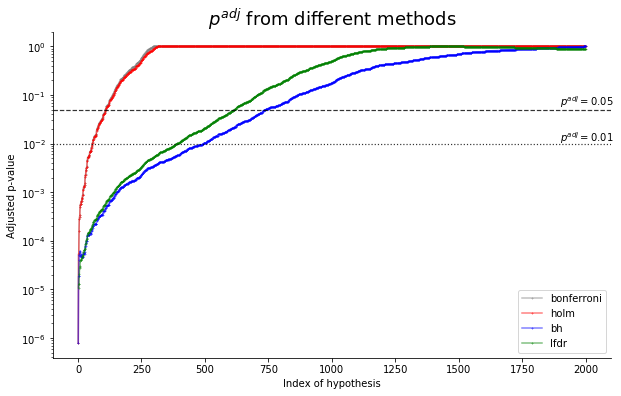
\includegraphics[scale=0.5]{adj_pval}
}

\frame
{
    \frametitle{\LARGE Simulation \& Comparison}
    \normalsize
    \begin{table}
      \small
      \setlength{\tabcolsep}{3pt}
    \begin{tabularx}{\hsize}{@{}l LLL@{}}
        \toprule
     & Bonferroni  & Holm & B-H \\
        \midrule
    True rejection
        & 107
            & 109
                & \textbf{721}\\
    False rejection 
        &  1
            & 1
                & 18 \\
    Total rejection
        & 108
            & 110
                &  739   \\
    \midrule
    Ratio of false rejection 
            & .009
                & .009
                    & \textbf{.014}    \\
    Ratio of true acception 
            & .529
                & .529
                    & .780    \\
        \bottomrule
      \end{tabularx}
      \caption{simulation result at $FWER \leq 0.05$ or $FDR \leq 0.05$}
    \end{table}
}


% REFERENCES
\frame
{
    \frametitle{\LARGE References}
    \scriptsize
    \begin{itemize}
    \item Savin, N. (1980). "The Bonferroni and the Scheff\'e Multiple Comparison Procedures". The Review of Economic Studies, 47(1), 255-273\\
\item Weisstein, E. "Bonferroni Inequalities". From \href{http://mathworld.wolfram.com/BonferroniInequalities.html}{MathWorld - A Wolfram Web Resource}, retrieved at Dec. 2017
\item Holm, S. (1979). "A Simple Sequentially Rejective Multiple Test Procedure". Scandinavian Journal of Statistics, 6(2), 65-70\\
\item Abdi, H. (2010). "Holm's Sequential Bonferroni Procedure". University of Texas at Dallas\\
\item Aickin, M., Gensler, H. (1996). "Adjusting for multiple testing when reporting research results: the Bonferroni vs Holm methods". American Journal of Public Health, 86(5), 726?728\\
\item Benjamini, Y., Hochberg, Y. (1995). "Controlling the False Discovery Rate: A Practical and Powerful Approach to Multiple Testing". Journal of the Royal Statistical Society. Series B (Methodological), 57(1), 289-300\\
\item Benjamini, Y., Yekutieli, D. (2001). "The control of the false discovery rate in multiple testing under dependency". Ann. Statist. 29(4), 1165-1188\\
\item Robinson, D. (2015). "Understanding empirical Bayes estimation (using baseball statistics)". From \href{http://varianceexplained.org/r/empirical\_bayes\_baseball/}{Variance Explained}, retrieved at Dec. 2017 \\
\item Efron, B., Tibshirani, R., Storey, J., Tusher, V. (2001). "Empirical Bayes Analysis of a Microarray Experiment". Technical Report. 216\\
    \end{itemize}
}

\end{document}
